\begin{solution}
This problem is called the Prince Rupert's cube problem. The length of the largest cube that can go through the original cube is $\frac{3\sqrt{2}}{4} \approx 1.0606601$.\\[0.2cm]

Place two points on two adjacent edges of a unit cube, each at a distance of 3/4 from the point where the two edges meet, and two more points symmetrically on the opposite face of the cube. Then these four points form a square with side length
$\frac{3\sqrt{2}}{4} \approx 1.0606601.$

\begin{center}
	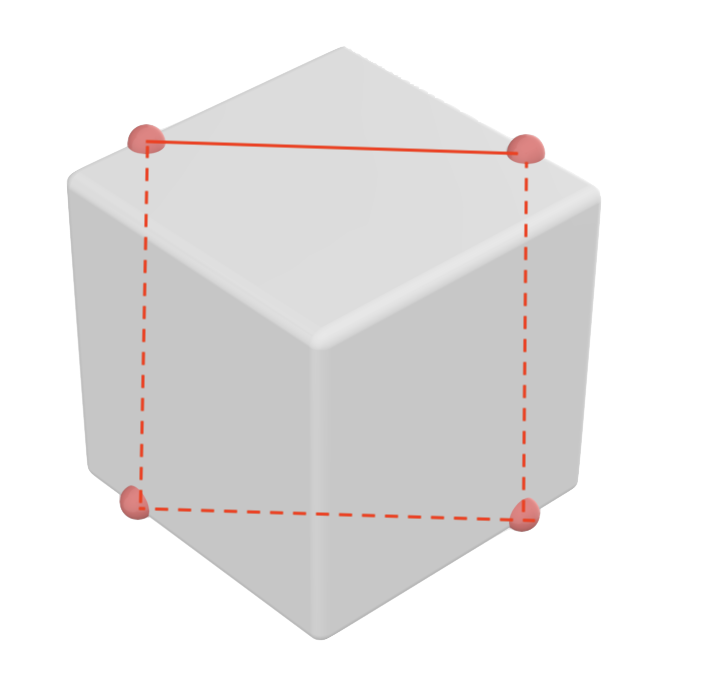
\includegraphics[width=5cm]{51/figs/51_sol1.png}
\end{center}

Notice that these four points make a square of length $(3\sqrt{2})/4$. Extruding the square in both directions perpendicularly to itself forms the hole through which a cube larger than the original one, up to side length $(3\sqrt{2})/4$, may pass.

\end{solution}